% ------------------------------------------------------------------------------
% TYPO3 CMS 7.3 - What's New (German Version)
%
% @author	Patrick Lobacher <patrick@lobacher.de> and Michael Schams <schams.net>
% @license	Creative Commons BY-NC-SA 3.0
% @link		http://typo3.org/download/release-notes/whats-new/
% @language	German
% ------------------------------------------------------------------------------
% LTXE-CHAPTER-UID:		cc6b358d-f0ed36d3-f7a72fa2-af63ccfc
% LTXE-CHAPTER-NAME:	Backend User Interface
% ------------------------------------------------------------------------------

\section{Backend User Interface}
\begin{frame}[fragile]
	\frametitle{Backend User Interface}

	\begin{center}\huge{Kapitel 1:}\end{center}
	\begin{center}\huge{\color{typo3darkgrey}\textbf{Backend User Interface}}\end{center}

\end{frame}

% ------------------------------------------------------------------------------
% LTXE-SLIDE-START
% LTXE-SLIDE-UID:		b4dc1576-57b4854f-26a32d85-11f7c52b
% LTXE-SLIDE-TITLE:		Feature #66173: Allow page title edit by doubleclick
% LTXE-SLIDE-REFERENCE:	Feature-66173-AllowPageTitleEditByDoubleclick.rst
% ------------------------------------------------------------------------------
\begin{frame}[fragile]
	\frametitle{Backend User Interface}
	\framesubtitle{Seitentitel im Page- und List-Modul}

	Im Page- und List-Modul kann man den Seitentitel entweder per Doppelklick
	oder mit Klick auf das Bearbeitungssymbol ändern.

	\begin{figure}
		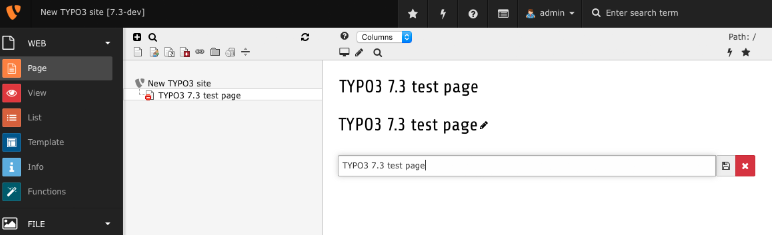
\includegraphics[width=0.9\linewidth]{BackendUserInterface/66173.png}
	\end{figure}

\end{frame}

% ------------------------------------------------------------------------------
% LTXE-SLIDE-START
% LTXE-SLIDE-UID:		168b1424-1ebb2552-ed5bac3e-8a9ac737
% LTXE-SLIDE-TITLE:		Feature #67071: Processed files cleanup tool added in Install Tool
% LTXE-SLIDE-REFERENCE:	Feature-67071-ProcessedFilesCleanupToolAddedInInstallTool.rst
% ------------------------------------------------------------------------------
\begin{frame}[fragile]
	\frametitle{Backend User Interface}
	\framesubtitle{Prozessierte FAL Dateien im Install Tool löschen}

	Das Install Tool enthält nun ein neues Tool (unterhalb von "Clean up"), um
	prozessierte FAL Dateien (wie z.B. Thumbnails) zu löschen. Das ist
	insbesondere hilfreich, wenn man grafik-relevante Settings ändern oder wenn
	man GraphicsMagick/ImageMagick aktualisiert hat und alle Dateien neu
	generieren will.

	\begin{figure}
		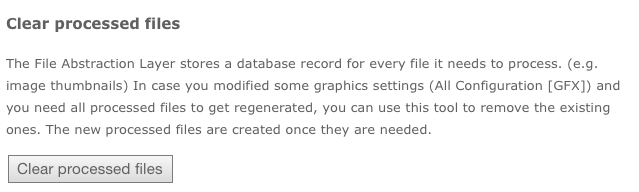
\includegraphics[width=0.6\linewidth]{BackendUserInterface/67071.png}
	\end{figure}

\end{frame}

% ------------------------------------------------------------------------------
% LTXE-SLIDE-START
% LTXE-SLIDE-UID:		daa83c1e-08d2716b-de74cbda-42361551
% LTXE-SLIDE-TITLE:		Feature #67319: Add field "copyright" to EXT:filemetadata
% LTXE-SLIDE-REFERENCE:	Feature-67319-AddFieldCopyrightToEXTfilemetadata.rst
% ------------------------------------------------------------------------------
\begin{frame}[fragile]
	\frametitle{Backend User Interface}
	\framesubtitle{Copyright in FAL Meta-Daten}

	In den zusätzlichen FAL Meta-Daten (Extension: \texttt{filemetadata}) gibt
	es nun ein Feld "\textbf{Copyright}".

	\begin{figure}
		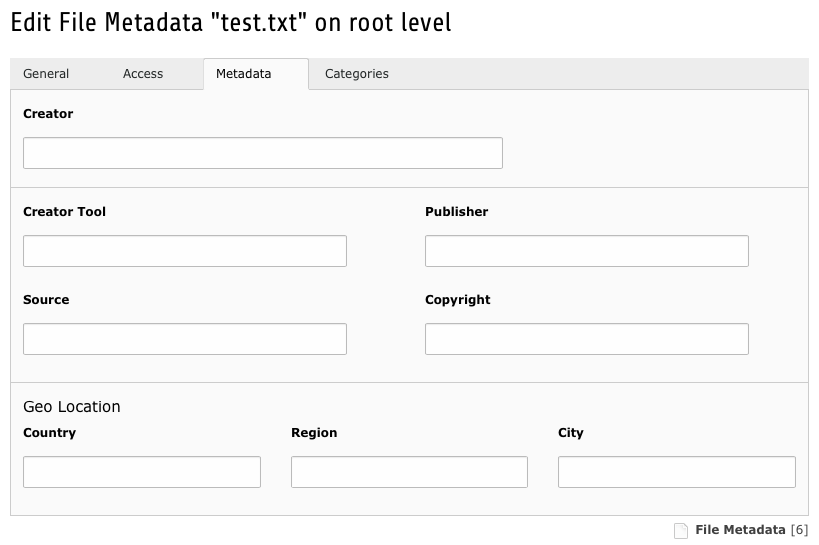
\includegraphics[width=0.6\linewidth]{BackendUserInterface/67319.png}
	\end{figure}

\end{frame}

% ------------------------------------------------------------------------------
